% Drafted against audit/outline.md §7. Two deviations, both recorded in the
% outline: the sweeps table appears first (Table 8) and the candidate ledger
% second (Table 9), because the sweep is the evidence and the ledger is the
% summary; and the "tested at the disclosed settings, and refuted" subsection
% is new since the original outline, which predates the discovery that the
% disclosed window and weighting had never been implemented.
%
% Evidence: robustness_windows.csv, robustness_age_weighting.csv,
% robustness_sign_variants.csv, robustness_percentile.csv,
% convexity_comparison.csv, disclosed_var_commentary.csv, hash-recorded in
% audit/evidence_freeze.csv at commit 1e6bdd74.

\section{Which assumptions can explain the gap}\label{sec:assumptions}

Section~\ref{sec:results} established a gap: the disclosed diversification
effect moves by 2.08 percentage points a year and the proxy book's moves by
6.33. This section works through what could account for it, candidate by
candidate, and reports which survive.

\subsection{Ruled out by magnitude}

Two specification choices can be dismissed by size alone, without any argument
about mechanism.

The percentile convention is one. Reading the loss quantile by linear
interpolation rather than as a discrete order statistic moves average VaR by
0.30\% and the mean diversification ratio by 0.06 percentage points. Convexity
is the other. Pricing the rate sleeve by full revaluation rather than by a
duration approximation moves annual average VaR by between 0.25\% and 0.59\%,
with a largest single-day gap of 1.55\%. Neither is within two orders of
magnitude of a four-point discrepancy in a ratio's standard deviation.

Both are worth running anyway, because an unexamined choice is an unexamined
choice, and because the convexity comparison establishes something useful in
its own right: on a one-day horizon with daily yield moves of about five basis
points, full revaluation on vanilla bonds buys three tenths of a percent. It
earns its cost on instruments whose value is sharply non-linear in the factor,
which means options, and on longer horizons. That is a finding about method
rather than about Goldman.

\subsection{Right direction, not far enough}

The scenario window is a real effect and the first candidate that moves the
result.

The top block of Table~\ref{tab:sweeps} runs the window at one, two, three and
five years with equal weights. Steadiness improves monotonically as the window
lengthens: the year-to-year standard deviation falls from 10.23 points at one
year to 8.87 at two, 8.36 at three and 6.33 at the disclosed five. The level
climbs toward the disclosure at the same time, from 38.2\% to 41.6\% against
42.0\%.

% Generated by build/make_tables.py from robustness_windows.csv and robustness_age_weighting.csv. Do not edit.

\begin{table}[tbp]
\centering
\small
\caption{Steadiness and coverage move in opposite directions under Goldman's own disclosed settings}
\label{tab:sweeps}
\begin{tabular}{@{}llrrrr@{}}
\toprule
 & Half-life & Mean & Year-to-year & Exception & \\
Specification & (days) & (\%) & std.\ dev.\ (pp) & rate (\%) & Kupiec \\
\midrule
\multicolumn{6}{@{}l}{\emph{Lookback window, equally weighted}} \\
252 days (1y) & --- & 38.2 & 10.23 & 5.58 & 0.209 \\
502 days (2y) & --- & 39.0 & 8.87 & 5.58 & 0.209 \\
756 days (3y) & --- & 39.6 & 8.36 & 5.89 & 0.058 \\
1,260 days (5y)\;$\dagger$ & --- & 41.6 & 6.33 & 6.98 & $<$0.0001 \\
\addlinespace
\multicolumn{6}{@{}l}{\emph{Scenario age weighting, at the disclosed window}} \\
$\lambda = 1.00$ (equal) & --- & 41.6 & 6.33 & 6.98 & $<$0.0001 \\
$\lambda = 0.99$ & 69 & 39.9 & 10.04 & 5.45 & 0.328 \\
$\lambda = 0.97$ & 23 & 42.0 & 9.46 & 5.63 & 0.177 \\
\midrule
\emph{Goldman, as disclosed} & --- & 42.0 & 2.08 & 0.40 & --- \\
\bottomrule
\end{tabular}
\notetext{$\dagger$ marks the disclosed window. The top block holds the weighting equal and varies the window length; the lower block holds the window at the disclosed five years and varies the decay. Reading down the lower block, the year-to-year standard deviation rises while the exception rate falls toward its nominal 5\% and Kupiec stops rejecting: adopting Goldman's disclosed weighting makes the engine a better risk model and a worse reproduction of the disclosed steadiness, at the same time. Goldman's own exception rate is measured against net revenues and is not comparable; it is shown for scale only and discussed in Section~\ref{sec:results}.}
\end{table}


The direction is right and the destination is not. Five years is the end of
this road rather than a point along it, because five years is what Goldman
discloses: there is no longer window to appeal to. At the disclosed length
the ratio still moves three times as much as the disclosed series, and the
engine's coverage has deteriorated badly in the process: the exception rate
rises from 5.58\% at one year to 6.98\% at five, and Kupiec goes from not
rejecting to rejecting below any conventional level. A five-year equally
weighted scenario set is slow, and 2022 is where that shows: 70 exceptions in
230 trading days, because five years of scenarios in early 2022 reached back
to 2017 and contained almost no rate volatility.

\subsection{Tested at the disclosed settings, and refuted}

The obvious objection to everything above is that a seventeen-factor proxy is a
blunter instrument than Goldman's, so the gap measures the replication rather
than the bank. The disclosed age weighting tests that objection directly,
because it is the one remaining piece of Goldman's stated method that had not
been applied, and because it bears on exactly the quantity in dispute: how
quickly the engine's view of the correlation structure turns over.

It does not close the gap. It widens it. The lower block of
Table~\ref{tab:sweeps} holds the window at the disclosed five years and varies
the decay. At a 69-day half-life the year-to-year standard deviation rises from
6.33 to 10.04 points; at a 23-day half-life, to 9.46. Against a disclosed 2.08,
adopting Goldman's own weighting takes the engine from three times too variable
to four or five times too variable.

And it does so while making the engine a better risk model by every coverage
test applied to it. The exception rate falls from 6.98\% to 5.45\% at the
longer half-life and 5.63\% at the shorter, both close to the nominal 5\%.
Kupiec's $p$-value rises from below 0.0001 to 0.328 and 0.177 respectively, and
at the faster decay the independence test passes as well, at 0.305. Weighting
toward recent observations is the correct specification for a
historical-simulation engine; the filings say so in plain terms, and the
backtest agrees with them.

The two movements are in opposite directions and that is the point. Reading
down the lower block of Table~\ref{tab:sweeps}, coverage improves and
steadiness degrades together. The gap between the disclosed steadiness and the
reproduced steadiness is therefore not an artefact of this replication using a
cruder method than the bank. It uses the bank's method, the bank's own window
and weighting scheme, and the gap gets larger.

The filings disclose the weighting in kind but not in degree: they say the
importance of the data reduces over time without giving the rate. Two rates
cannot establish what every rate would do, so the parameter was swept across
sixteen values spanning half-lives from 6.6 trading days to 1{,}386, and
Figure~\ref{fig:decay} reports the result.

The relationship is not monotone, which is worth saying plainly because the
obvious argument, that faster decay turns the scenario set over faster and
so must increase variability, is wrong. Year-to-year variability rises
steeply as decay is introduced, peaks at 10.04 points around a 69-day
half-life, and then falls back to 8.65 at the fastest rate tested. The
conclusion survives the correction and is now demonstrated rather than
asserted: the steadiest configuration anywhere in the grid is equal weighting
itself, at 6.33, and every weighted configuration is further from the
disclosures than that. The minimum across all sixteen rates is three times
Goldman's 2.08.

\begin{figure}[tbp]
\centering
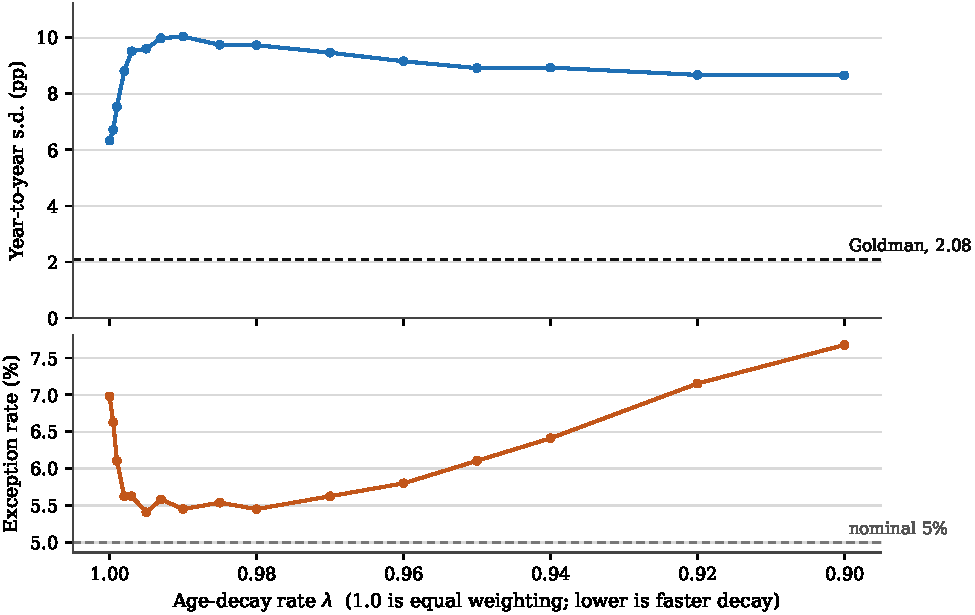
\includegraphics[width=\linewidth]{figures/decay_grid}
\caption{Year-to-year variability and coverage against the age-decay rate, at
the disclosed five-year window. Sixteen rates, from equal weighting to a
6.6-day half-life. The upper panel never approaches Goldman's 2.08 anywhere in
the grid, and its minimum is equal weighting. The lower panel reaches the
nominal 5\% exception rate in the middle of the range, where the upper panel
is near its worst.}
\label{fig:decay}
\end{figure}

The lower panel shows the opposing movement across the whole grid rather than
at two points. Coverage is best near a 138-day half-life, where the exception
rate is 5.41\% against a nominal 5\% and Kupiec's $p$-value reaches 0.376,
and the year-to-year variability there is 9.61, among the worst in the sweep.
There is no rate at which the engine is both well calibrated and as steady as
the disclosures, and the sweep is dense enough to say so.

\subsection{Bounded by the configuration space}

Sleeve direction remains the specification choice with the largest effect on
the diversification effect, and Section~\ref{sec:results} reported the bound:
across all sixteen sign configurations, five are at least as steady as the
disclosure and the best of those averages 35.6\%, while eight reach 40\% or
more and the steadiest of those varies by 3.68 points. None does both.

What that bound rules out is a particular kind of objection: that the long-only
baseline is simply the wrong corner of the space, and some other corner would
land on Goldman. It would have to be a corner that is not in the space. The
sixteen configurations exhaust the sign choices available to a four-sleeve
book, and the empty quadrant in Figure~\ref{fig:frontier} is a property of all
of them.

\subsection{What survives}

Three candidates the frozen evidence cannot exclude, and they are not ranked,
because nothing here ranks them.

\emph{The factor count.} Seventeen factors against the roughly 70,000 the
FY2016 and FY2017 filings describe. More independent sources of risk means more
diversification available, so the direction of the bias on the \emph{level} is
known. The direction on the \emph{steadiness} is not: a larger factor set might
average out regime shifts in any one correlation, or might not. Nothing in
public data settles it, and this paper does not guess.

\emph{Non-synchronous closes.} Tokyo, London and New York do not close at the
same instant, which depresses measured cross-market correlation and therefore
overstates diversification. This runs opposite to the factor-count bias, which
is why neither is used to argue the result in either direction. Neither is
quantified.

Table~\ref{tab:candidates} summarises the three verdicts below alongside the
exclusions above.

\emph{Exposure management.} This is the candidate with direct evidence behind
it, and Section~\ref{sec:results} sharpened what it has to explain. A static
book cannot reproduce a path produced by a desk that trades against the market,
and Goldman's own commentary says that is what the desk does. In four
consecutive filings --- FY2021 through FY2024 --- the explanation of the
year-over-year VaR change has the same shape: volatility moved one way,
``partially offset by'' exposures moving the other. The firm also moved
positions in and out of the measure outright, as the first-quarter 2023 scope
change shows. A book whose notionals were fixed in 2019 has no counterpart to
any of that.

What Table~\ref{tab:amplitude} adds is that this candidate now has a specific
job. It does not need to explain why Goldman's ratio moves less than the
proxy's, because on a like-for-like basis it does not: period-end against
period-end the two have almost the same year-to-year variation. It needs to
explain why Goldman's movements revert and the proxy's accumulate. Exposure
management is a mechanism that would do exactly that. A desk that sells risk
into a correlation regime it dislikes and buys it back when the regime passes
produces a ratio that wanders and returns; a fixed book exposed to the same
market produces one that wanders and stays. Nothing in the public data
establishes that this is what happens, but of the three surviving candidates it
is the only one whose mechanism matches the shape of the discrepancy.

% Generated by build/make_tables.py from the robustness and comparison outputs. Do not edit.

\begin{table}[tbp]
\centering
\footnotesize
\setlength{\tabcolsep}{5pt}
\caption{Candidate explanations for the steadiness gap, and what settles each}
\label{tab:candidates}
\begin{tabularx}{\linewidth}{@{}l Y l@{}}
\toprule
Candidate & What settles it & Verdict \\
\midrule
Percentile convention & Moves VaR by 0.30\% and the mean ratio by 0.06 pp & Excluded \\
Convexity in the rate sleeve & Full revaluation against duration moves annual VaR by at most 0.59\% & Excluded \\
Lookback window too short & Lengthening 1y$\rightarrow$5y cuts the gap from 10.23 to 6.33 pp, against 2.08 & Right way, insufficient \\
Equal weighting, not Goldman's & Swept over 16 decay rates: the steadiest is equal weighting at 6.33 pp and every weighted rate is worse, while coverage improves & Refuted \\
Wrong sleeve directions & Of 16 configurations, 5 match the steadiness and peak at 35.6\%; 8 match the level and bottom out at 3.68 pp & Excluded \\
Seventeen factors, not 70{,}000 & Not testable on public data; biases the level downward, direction on steadiness unknown & Survives \\
Non-synchronous closes & Depresses measured cross-market correlation; magnitude not estimated & Survives \\
Exposures are managed, not held & Goldman attributes VaR changes to exposure moves in four consecutive filings; the only candidate whose mechanism produces reversion rather than drift & Survives \\
\bottomrule
\end{tabularx}
\notetext{The disclosed year-to-year standard deviation is 2.08 percentage points; every quantity in the middle column is measured against that. \emph{Refuted} is stronger than \emph{excluded}: the disclosed weighting was adopted and moved the gap the wrong way. The three surviving candidates are not ranked, because nothing in the frozen evidence ranks them.}
\end{table}


\subsection{Taken together}

The gap survives the removal of every specification choice that could be
removed. It is not the percentile rule, not convexity, not the window length,
not the weighting scheme, and not the sleeve signs. What remains is structural:
a static four-sleeve book exposed to seventeen public factors, against a
trading operation with a far larger factor set that repositions daily.

It is worth restating what the gap is, now that Section~\ref{sec:results} has
narrowed it. The proxy is not insufficiently variable or excessively variable
relative to the disclosures; measured on the same basis its variation is almost
identical in size. The proxy's variation persists where Goldman's reverts, and
every candidate above has been tested against that discrepancy rather than
against a difference in amplitude that does not exist.

\citet{danielsson2016modelrisk} give the mechanism in general form. Model risk,
the tendency of different models to disagree, rises with market
uncertainty: candidate models agree in calm periods and diverge significantly
in distress. Read through the diversification ratio, that is what
Section~\ref{sec:results} reports. The proxy tracks the disclosure closely
through the calm years to 2021, and separates from it in 2022 and after.
Their object is risk forecasts in general rather than a disclosed
diversification effect, so this is an application of their finding rather than
a confirmation of it.

The reading this paper settles on is narrow by design. A static book cannot
hold a diversification ratio near 42\% through both 2021 and 2023, because the
correlation structure beneath it changed and the book did not. Goldman's did
hold. Whatever accounts for that is not in the methodology the filings
disclose, because the methodology the filings disclose has been applied here
and does not produce it.
